% \chapter*{Erkl\"arung}
%%\vspace{10cm}
%Hiermit versichere ich, dass ich die vorliegende Masterarbeit
%selbstst\"andig verfasst und keine anderen als die angegebenen Quellen und Hilfsmittel
%verwendet habe. Alle Textausz\"uge und Grafiken, die sinngem\"a\ss\ oder
%w\"ortlich aus ver\"offentlichten Schriften entnommen wurden, sind durch
%Re\-fe\-ren\-zen ge\-kenn\-zeichnet.%\cite{peitz:2010} \\[3ex]
% 
% Hiermit versichere ich, diese Arbeit selbstständig verfasst zu haben und keine anderen als die angegebenen Quellen und Hilfsmittel benutzt sowie Zitate kenntlich gemacht zu haben. \\[3ex]
% 
% Aachen, \publicationDate\\[7ex]
% 
% Arne Nix

%%% Local Variables: 
%%% mode: latex
%%% TeX-master: "da"
%%% End: 
% \@openrighttrue


\chapter*{Erkl\"arung}
\vfill
% \vspace{2cm}
% \pagenumbering{gobble}
% \begin{center}
\begin{tikzpicture}[overlay, text height=1.5ex, text depth=0.25ex, yshift=0.5mm]
\node[anchor=south west,inner sep=0] at (0,0)  {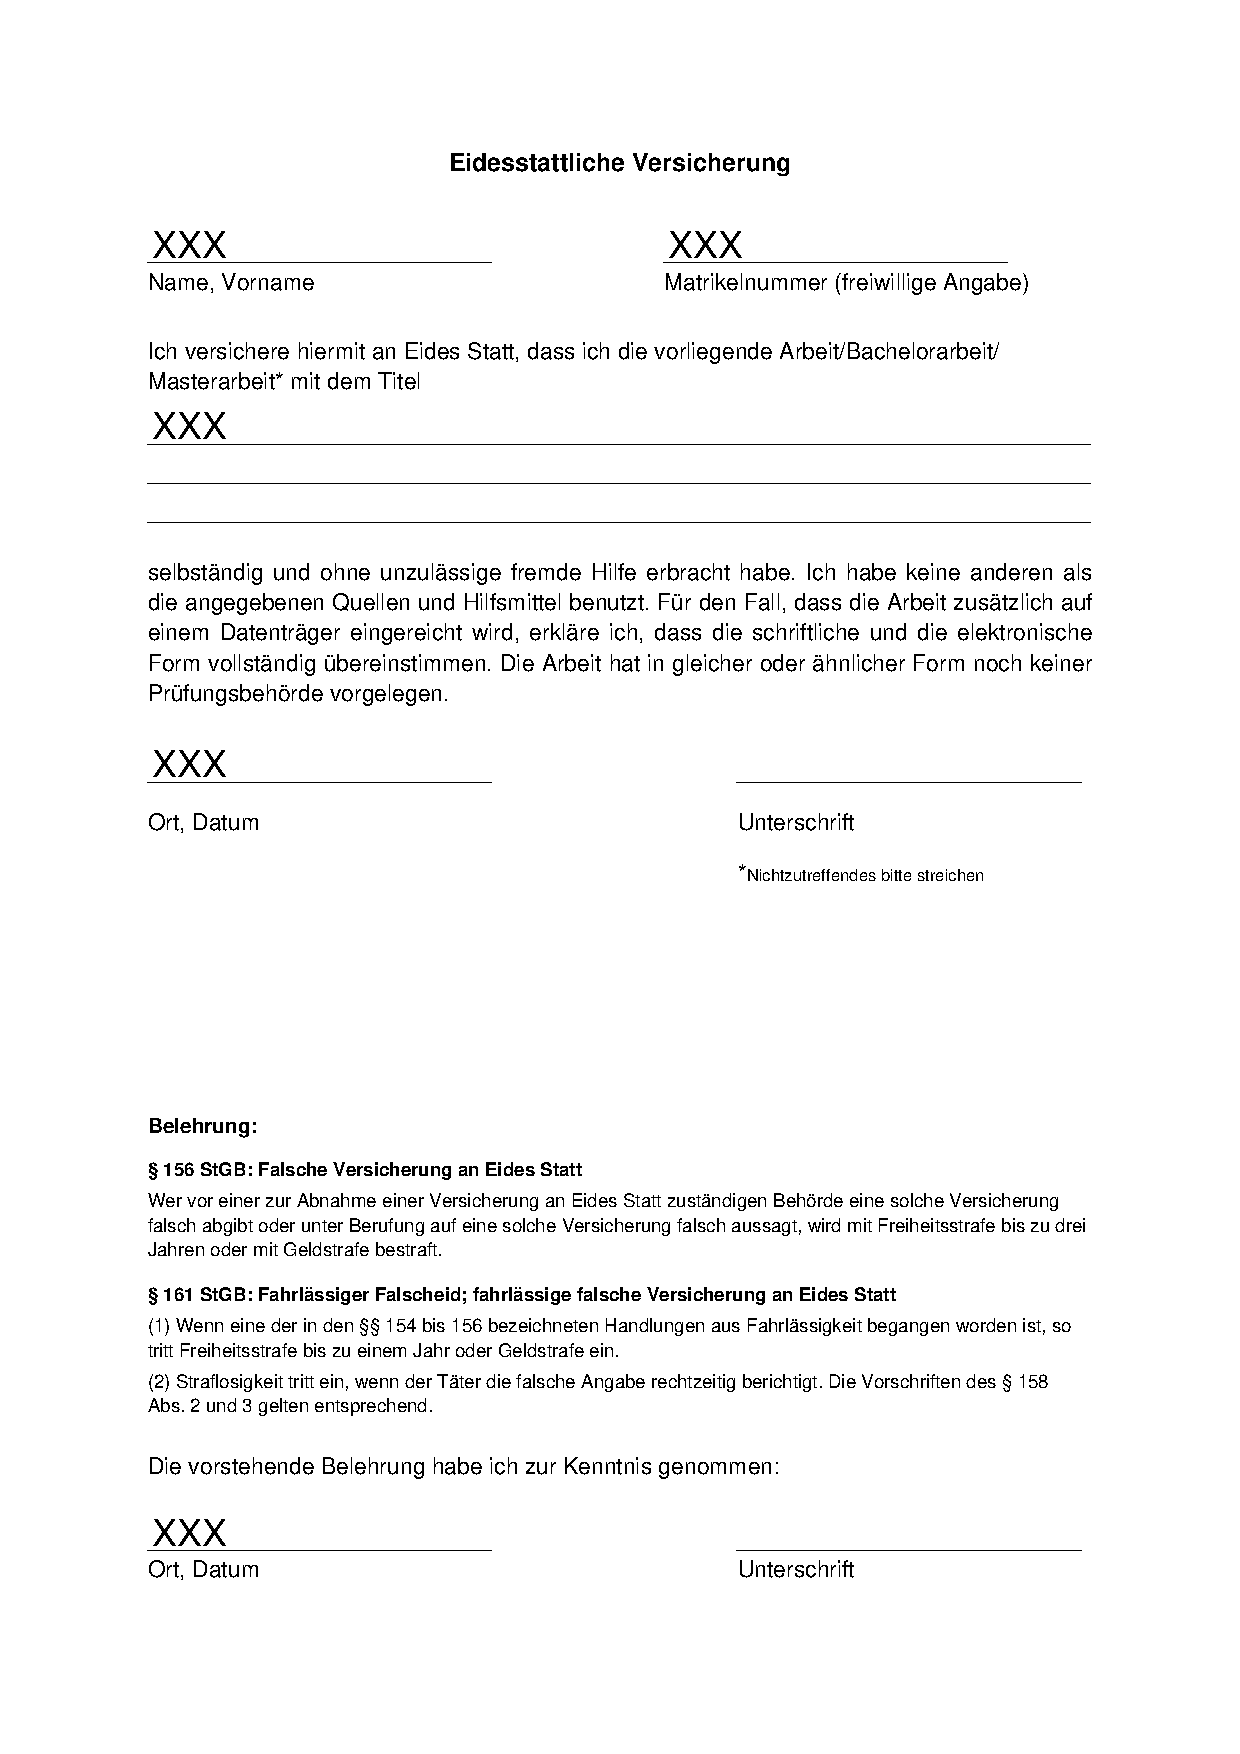
\includegraphics[width=0.95\linewidth, trim={2.5cm 3cm 2.5cm 4cm}, clip]{Formular_Eidesstattliche_Versicherung}};
\node [anchor=south west, inner sep=0] at (0cm, 18.4cm) {\Large \Surname, \Firstname};
\node [anchor=south west, inner sep=0] at (7.2cm, 18.4cm) {\Large \MatrikelNummer};
\node [anchor=south west, inner sep=0] at (0cm, 15.9cm) {\large \makeatletter \@title \makeatother};
\node [anchor=south west, inner sep=0] at (0cm, 11.2cm) {\large \Aachen, \publicationDate};
\node [anchor=south west, inner sep=0] at (0cm, 0.5cm) {\large \Aachen, \publicationDate};
\draw [line cap=round, line width=0.5mm] (8.8cm, 17.11cm) -- (9.65cm, 17.11cm); % cross out "Arbeit"
\draw [line cap=round, line width=0.5mm] (9.75cm, 17.11cm) -- (11.70cm, 17.11cm); % cross out "Arbeit"
%\draw [line cap=round, line width=0.5mm] (0cm, 16.7cm) -- (1.8cm, 16.7cm); % cross out "Masterarbeit"
\end{tikzpicture}
% \end{center}


% \includegraphics[width=0.95\linewidth, trim={2.5cm 2.9cm 2.5cm 3.9cm}, clip]{Formular_Eidesstattliche_Versicherung_neu}
